\Chapter{}
\chapter{CRONOGRAMA DE ACTIVIDADES}
    \begin{figure}[H] 
        \caption{\doublespacing \\ \textit{Cronograma de actividades para la investigación.}} 
        \centering
        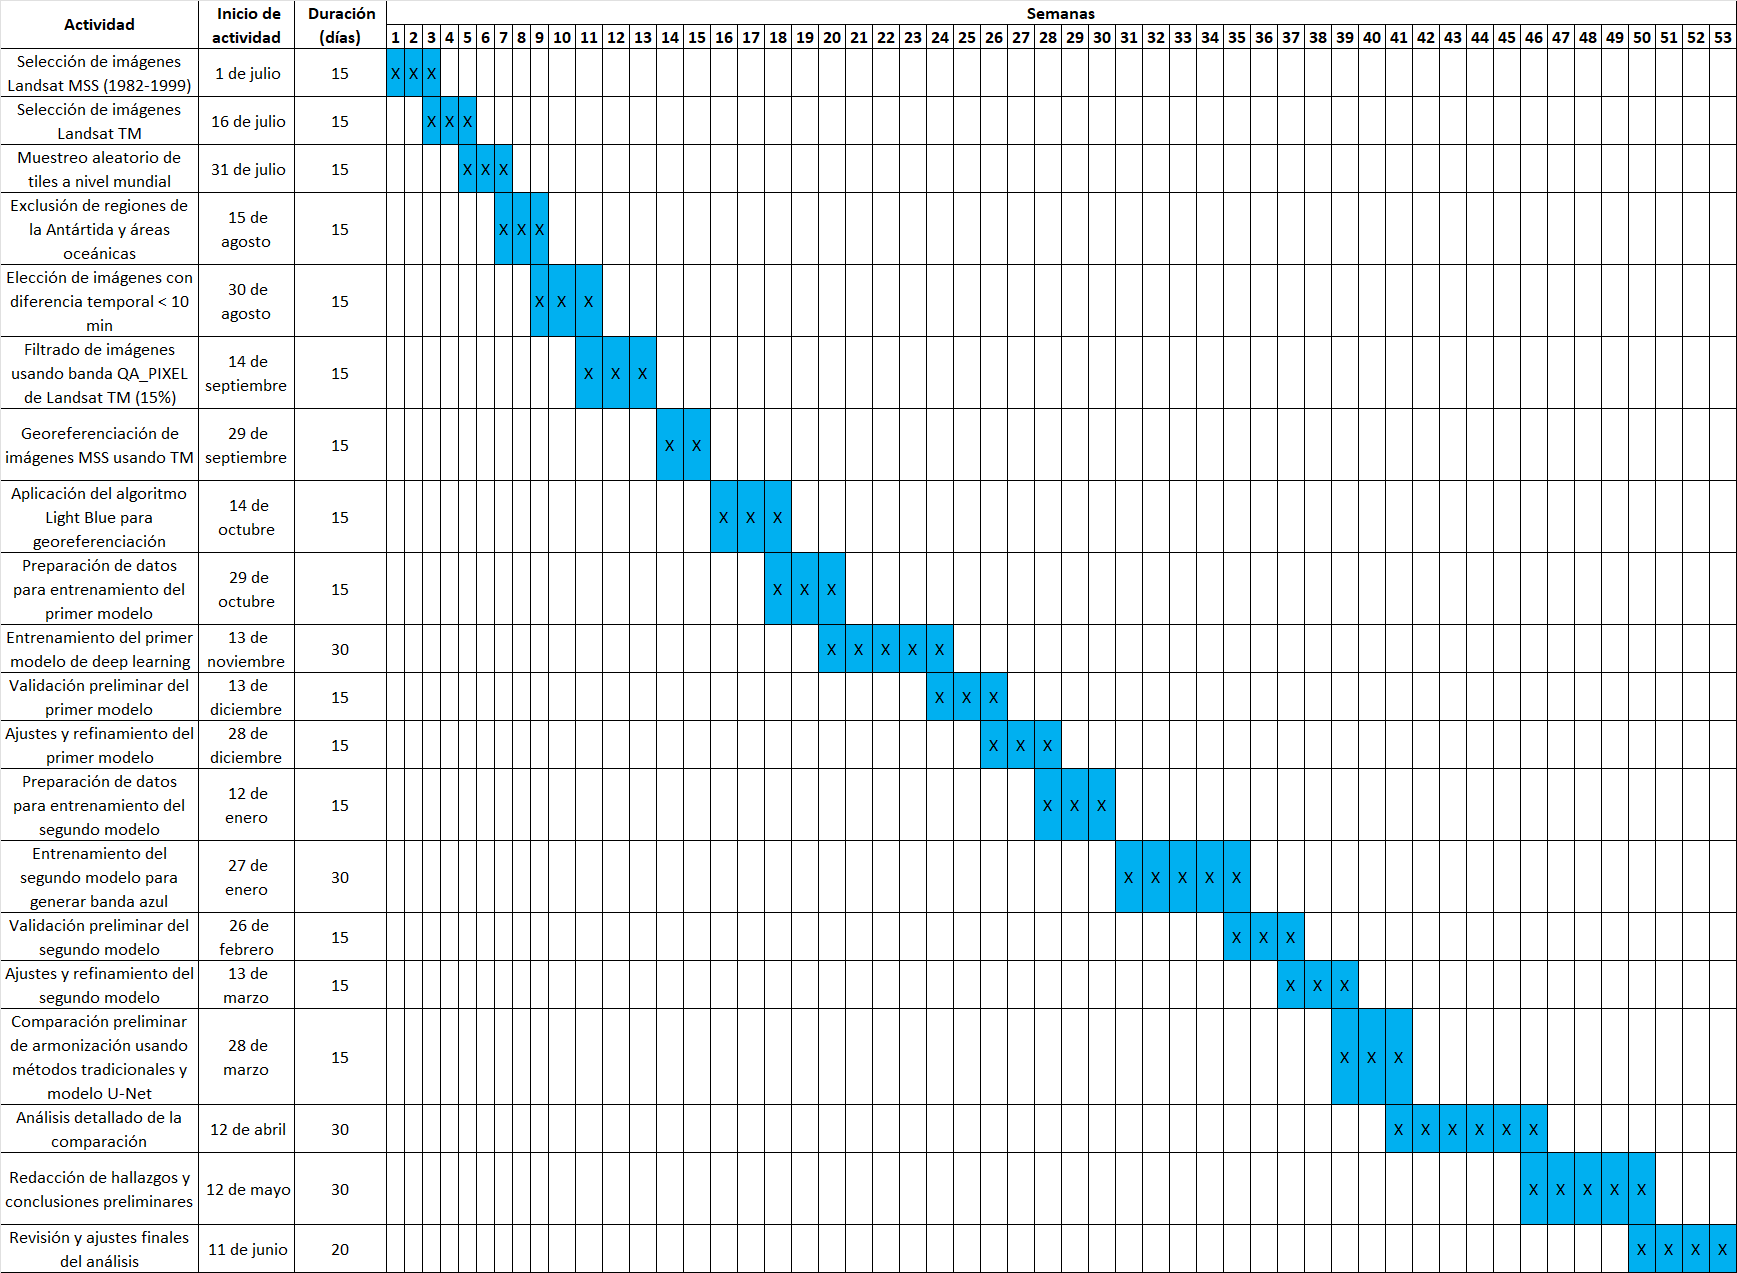
\includegraphics[width=1.12\linewidth, angle=90]{2_CAPITULO0/IMG/cronograma.png}
        \begin{justify}
            \textit{Nota.} El cronograma anual detalla la secuencia de actividades, desde la elección de imágenes Landsat hasta las modificaciones finales, organizadas semanalmente a lo largo de un año.
        \end{justify}                    
        \label{cronograma}
    \end{figure}

% \chapter{DISCUSIÓN}
%     La validación cuantitativa del modelo SWINIR - MSS2TM GAN se ejecutó con un enfoque en la precisión espectral y la superresolución, seleccionando estratégicamente Perú por su diversidad topográfica y ecosistémica. La comparativa con trabajos anteriores, reflejada en dos estudios significativos del campo, revela que el modelo exhibe un rendimiento competitivo, logrando una precisión en la superresolución que se alinea con los avances más recientes en la literatura.

%     La evaluación detallada de las métricas MAE, RMSE y el coeficiente de Pearson resalta el buen rendimiento general del modelo. Sin embargo, se identificaron variaciones en la efectividad de la superresolución entre diferentes áreas geográficas. Específicamente, la imagen 06008, ubicada sobre el Lago Titicaca, mostró valores elevados de MAE y RMSE, junto con un coeficiente de Pearson más bajo. Estos resultados sugieren que el modelo puede ser susceptible a errores inducidos por interferencia atmosférica y a desafíos inherentes a áreas con poca variación espectral, como las masas de agua.

%     Las implicaciones prácticas de los resultados son prometedoras, especialmente para aplicaciones que requieren alta fidelidad en la interpretación de datos satelitales. La exactitud en la superresolución de imágenes MSS se traduce en beneficios para la cartografía, la gestión de recursos naturales y la monitorización ambiental. No obstante, las limitaciones observadas apuntan a la necesidad de un tratamiento especializado de las imágenes sobre cuerpos de agua y áreas con condiciones atmosféricas adversas.